\documentclass{article}
\usepackage[utf8]{inputenc}
\usepackage[francais]{babel}
\usepackage{lmodern}
\usepackage[a4paper, margin=3cm]{geometry}
\usepackage{fancyhdr}

%Graphs and drawings
\usepackage{float}
\usepackage{circuitikz}
\usepackage{tikz}
\usepackage{tkz-graph}
\usepackage{subcaption}
\usetikzlibrary{decorations.pathreplacing}

%Math expressions
\usepackage{amsmath}
\usepackage{amsbsy}
\usepackage{breqn}

%Graphic expressions
\usepackage{graphicx}
\usepackage{wrapfig}

%Header
\pagestyle{fancy}
\fancyhf{}
\rhead{Éric Pfleiderer}
\fancyhead[L]{\leftmark}
\chead{}
\rfoot{}
\cfoot{\thepage}
 
\def\changemargin#1#2{\list{}{\rightmargin#2\leftmargin#1}\item[]}
\let\endchangemargin=\endlist 

\begin{document}

%Mise en page de la page titre
\begin{titlepage}
\center
\vspace*{2cm}
\textsc{\LARGE Université de Montréal}\\[1cm] 
\textsc{\Large PHY 3075 -- Modélisation numérique en physique}\\[4cm] %****éditer ceci***
\rule{\linewidth}{0.5mm} \\[0.5cm]
{\LARGE \bfseries Dispersion d'un polluant} \\[0.2cm] % ***éditer ceci***
{\LARGE \bfseries par advection-diffusion} \\[0.2cm]
\rule{\linewidth}{0.5mm} \\[4cm]
\large par: \\*
    Éric Pfleiderer \\* 
    20048976\\[4cm] 
{\large \today}\\[3cm]
\vfill
\end{titlepage}

\section*{Résumé}
%Objectif
L'objectif de ce laboratoire est de caractériser la nature d'un incident responsable de la dispersion d'un polluant. Le problème est modélisé à l'aide de l'équation de conservation incorporant un flux advectif, un flux diffusif et une source de polluant. La solution numérique est obtenue à l'aide des méthodes Leapfrog et Lax-Wendroff. On trouve par descente stochastique Monte Carlo que la position de la source polluante est de $(x_0, y_0) = (4.38\pm0.02,\ 2.65\pm0.02)$, tandis que son amplitude est de $S_0 = 1.82 \pm 0.09$. L'incident à débuté à $t_d = 0.09 \pm 0.006$ et s'est terminé à $t_f = 2.5$.

\section*{Introduction}

Le 11 mars 2011, un tsunami d'une envergure inattendue engendre des dommages catastrophiques à la station nucélaire de Fukushima Daiichi au Japon. Dans les jours qui suivent, un échec des systèmes de refroidissement mène à l'explosion de trois unités principales de la centrale. On assiste alors à la deuxième plus grande déversée de matériel radioactif dans l'histoire de l'humanité, suivant la catastrophe nucléaire de Tchernobyl en avril 1986.


L'objectif de ce laboratoire est de solutionner le problème de la dispersion d'un polluant en deux dimensions afin de déterminer l'emplacement et la nature d'un incident fictif similaire aux catastrophes de Tchernobyl et Fukushima. Le problème est modélisé par l'équation d'advection-diffusion et est solutionné numériquement à l'aide des méthodes Leapfrog et Law-Wendroff. On valide d'abord la calibration de ces méthodes en reproduisant des résultats connus. Ensuite, on détermine l'amplitude et l'emplacement de la source de polluant à partir de séquences temporelles fournies en implémentant une descente stochastique de type Monte Carlo.

\section{Théorie}
\subsection{Modélisation physique}\label{sec:model_physique}

Le problème de la dispersion d'un polluant se modélise à l'aide de l'équation de conservation (\ref{eq:conservation}), qui relie la variation temporelle d'une quantité à sa variation dans l'espace. 

\begin{equation}\label{eq:conservation}
\frac{\partial u}{\partial t} + \nabla \cdot (\textbf{F}) = 0
\end{equation}

La variation spatiale dépend de plusieurs facteurs dit passifs ou actifs. Par exemple, la diffusion est un phénomène de transport spontané et irréversible engendré par une différence de concentration entre deux milieux. Ce phénomène tend à homogéniser la composition d'un milieu et sa spontanéité est expliquée par une augmentation continuelle de l'entropie durant le processus \cite{thermodynamics}. La diffusion se modélise en substituant le flux diffusif $ \textbf{F} = -D \nabla u$ dans l'équation de conservation. En supposant que $D$ est constant dans l'espace, l'équation prend alors la forme (\ref{eq:conservation_flux_diffusif}). 

\begin{equation}\label{eq:conservation_flux_diffusif}
\frac{\partial u}{\partial t} + \nabla \cdot (-D \nabla u) = \frac{\partial u}{\partial t} - D \Big( \frac{\partial^2 u}{\partial x^2} + \frac{\partial^2 u}{\partial y^2} \Big) = 0
\end{equation}

La dispersion d'une substance dans l'espace peut aussi être attribuée à un phénomène d'advection, qui est simplement le déplacement naturel de la masse d'air qui contient le polluant. Le flux advectif prend la forme $F = \textbf{v} \ u$, ou $\textbf{v}$ est une fonction vectorielle qui décrit les courants d'air en tout points de l'espace étudié. En substituant le flux advectif dans l'équation de conservation, on obtient l'équation (\ref{eq:conservation_flux_advectif}).

\begin{equation}\label{eq:conservation_flux_advectif}
\frac{\partial u}{\partial t} + v_x (x,y,t) \frac{\partial u}{\partial x} + v_y (x,y,t) \frac{\partial u}{\partial y} = 0
\end{equation}

Finalement, les deux phénomènes peuvent être inclus dans le même modèle en sommant leur contribution respective. On ajoute aussi une source $S(x, y, t)$ qui décrit une contribution nette de polluant au système. L'équation qui modélise le problème de la dispersion d'un polluant par advection-diffusion en deux dimensions prend donc la forme finale (\ref{eq:conservation_finale}).

\begin{equation}\label{eq:conservation_finale}
\frac{\partial u}{\partial t} =  - v_x(x,y,t) \frac{\partial u}{\partial x} - v_y(x,y,t) \frac{\partial u}{\partial y} + D \Big(\frac{\partial^2 u}{\partial x^2} + \frac{\partial^2 u}{\partial y^2}\Big) + S(x,y,t)
\end{equation}

Durant l'ensemble du laboratoire, les fonctions décrivant l'advection et la source de polluant prennent la forme  (\ref{eq:forme}), où $t_d$ et $t_f$ représentent les bornes de l'intervalle de temps durant lequel la source émet activement du polluant.

\begin{equation} \label{eq:forme}
\begin{gathered}
v_x(x,y,t) = u_0\ A\ cos[y + \epsilon \ sin(wt)]\\
v_y(x,y,t) = u_0\ B\ cos[x + \epsilon \ sin(wt)]\\
\end{gathered}
\end{equation}
\begin{equation*}
S(x,y,t) = S_0 \ f(t) \ exp\big(\frac{-r^2}{w^2}\big), 
\hspace{1cm} r^2 = (x-x_0)^2 + (y-y_0)^2,
\hspace{1cm} f(t) = \begin{cases}
	1\ si\ t_d\ \leq \ t\ \leq t_f\ \\
	0\ sinon\\
\end{cases}
\end{equation*}

\section{Méthodologie}

\subsection{Analyse numérique}\label{sec:model_numerique}

Notre modèle d'advection-diffusion (\ref{eq:conservation_finale}) est une équation différentielle partielle d'ordre deux. Elle est solutionnée numériquement à l'aide de la méthode Leapfrog et de la méthode Lax-Wendroff. On commence par
discrétiser le temps et l'espace à l'aide des relations relations (\ref{eq:discretisation}), où $\Delta x$,  $\Delta y$ et $\Delta t$ sont les pas spatio-temporels de la solution. La variable $u_{j, k}^n$ représente alors la concentration du polluant à la position $(j, k)$ et au temps $n$.

\begin{equation}\label{eq:discretisation}
u_{j, k}^n, 
\hspace{1cm} n = \lfloor{\frac{t}{\Delta t}}\rfloor,
\hspace{1cm} j = \lfloor\frac{x}{\Delta x}\rfloor,
\hspace{1cm} k = \lfloor\frac{y}{\Delta y}\rfloor
\end{equation}

Dans le cadre des deux méthodes, la valeur des dérivées est évaluée numériquement à l'aide d'une série de Taylor tronquée au premier ordre (\ref{eq:taylor}).

\begin{equation}\label{eq:taylor}
f(t+ \Delta t) = f(t) + \Delta t \frac{df}{dt} + \mathcal{O}(t^2) \hspace{1cm} \longrightarrow \hspace{1cm} \frac{df}{dt} \approx \frac{f(t + \Delta t) - f(t)}{\Delta t}
\end{equation}

La méthode Leapfrog évalue les dérivées centrées dans l'espace et dans le temps. Dans le cadre de cette méthode, l'équation d'advection (\ref{eq:conservation_flux_advectif}) prend plutôt la forme (\ref{eq:adv_leapfrog}). Malheureusement, les erreurs de troncations s'accumullent rapidement sous Leapfrog et peuvent engendrer des oscillations dans la solution obtenue. Cette méthode est donc surtout utilisée à fins d'explorations initiales plutôt que pour détailler une solution exacte.

\begin{equation}\label{eq:adv_leapfrog}
\frac{ u_{j, k}^{n+1} - u_{j, k}^{n-1} }{2 \Delta t} = - v_x \frac{ u_{j+1, k}^{n} - u_{j-1, k}^{n} }{2 \Delta x} - v_y \frac{ u_{j, k+1}^{n} - u_{j, k-1}^{n} }{2 \Delta y}
\end{equation}

La méthode Lax-Wendroff, quant à elle, demande un temps de calcul additionnel mais réduit drastiquement l'accumulation des erreurs numériques. La première étape consiste à évaluer la solution à demi pas dans l'espace et dans le temps en incluant les flux désirés. L'équation (\ref{eq:lwsol_demipas}) montre une solution en une dimension spatiale incluant le flux advectif.

\begin{equation}\label{eq:lwsol_demipas}
	u_{j+\frac{1}{2}, k+\frac{1}{2}}^{n+\frac{1}{2}} = \frac{1}{4}(u_{j+1,k}^n + u_{j,k}^n + u_{j+1,k+1}^n + u_{j,k+1}^n) - \frac{\Delta t}{2} (v_x \frac{u_{j+1, k}^n - u_{j, k}^n}{\Delta x})
\end{equation}

La prochaine étape consiste à calculer le flux à demi pas dans le temps et dans l'espace à partir de la solution (\ref{eq:lwsol_demipas}). En incluant le flux diffusif, on obtient l'équation (\ref{eq:lwflux_demipas}), encore une fois seulement valide pour une dimension spatiale.

\begin{equation}\label{eq:lwflux_demipas}
	F_{j+\frac{1}{2},k+\frac{1}{2}}^{n+\frac{1}{2}} =  v_{j+\frac{1}{2},k+\frac{1}{2}}^{n+\frac{1}{2}} \ u_{j+\frac{1}{2},k+\frac{1}{2}}^{n+\frac{1}{2}} - \frac{D}{2 \Delta x} (u_{j+1, k}^{n} + u_{j+1, k+1}^{n}  - u_{j, k}^{n} - u_{j, k+1}^{n})
\end{equation}

Finalement, la solution à plein pas dans le temps est obtenue à partir de la solution précédente et des flux calculés à mis pas. L'équation (\ref{eq:lwsol_pleinpas}) résume l'ensemble des étapes discutés jusqu'à maintenant.

\begin{equation}\label{eq:lwsol_pleinpas}
	u_{j,k}^{n+1} = u_{j,k}^{n} - \frac{\Delta t}{2 \Delta x} (F_{j+\frac{1}{2},k+\frac{1}{2}}^{n-\frac{1}{2}} - F_{j+\frac{1}{2},k-\frac{1}{2}}^{n-\frac{1}{2}} + F_{j+\frac{1}{2},k+\frac{1}{2}}^{n+\frac{1}{2}} - F_{j-\frac{1}{2},k+\frac{1}{2}}^{n+\frac{1}{2}})
\end{equation}

La méthode de Lax-Wendroff se généralise facilement à plusieurs dimensions en y ajoutant les contributions nécéssaires. Les détails concernant les méthodes Leapfrog et Lax-Wendroff sont affichés dans le recueil de notes de Paul Charbonneau \cite{notes_cours}. 

\subsection{Descente stochastique de type Monte Carlo}

Notre objectif principale est de déterminer la nature du terme source ayant conduit à un certain incident. Plus spécifiquement, on cherche $S_0$, $x_0$, $y_0$ et $t_d$, soit l"amplitude, la position et le temps d'activation de la source. Les seules mesures disponibles concernant l'incident en question sont trois séquences temporelles de concentration associées aux points $(0.75 \times 2 \pi, 0.25 \times 2 \pi)$, $(0.5 \times 2 \pi, 0.5 \times 2 \pi)$ et $(0.25 \times 2 \pi, 0.75 \times 2 \pi)$. Pour quantifier la différence entre une solution possible et les séquences temporelles fournies, on utilise une différence de carrés (\ref{eq:moindres_carre}).

\begin{equation}\label{eq:moindres_carre}
	\chi^2 = \frac{1}{K} \sum_{k=1}^{K-1}(c_k^* - c(t_k))^2 
\end{equation}

Puisque notre solution doit prendre en compte simultanément les trois points de mesures, on définit une somme de différences de carrés qu'on désire optimiser (\ref{eq:fonction_min}), où les indices $1$, $2$ et $3$ dénottent les points de mesures.

\begin{equation}\label{eq:fonction_min}
	min\ \chi_1^2 + \chi_2^2  + \chi_3^2 
\end{equation}

L'optimisation de la fonction (\ref{eq:fonction_min}) est effectuée par descente stochastique de type Monte Carlo. L'algorithme débute avec un vecteur solution quelconque ainsi qu'une taille de pas caractéristique $h$. Une série de piges aléatoires provenant d'une distribution normale (\ref{eq:pige_normale}) sont alors entreprises pour chaque composante du vecteur solution. 

\begin{equation}\label{eq:pige_normale}
	pige\ stochastique \sim N(0, h)
\end{equation}

Les valeurs obtenues de la pige sont ajoutées à leur composante respective et un nouveau vecteur solution est ainsi généré. Si cette nouvelle solution optimise davantage la fonction (\ref{eq:fonction_min}), le vecteur est maintenu pour la prochaine itération de l'algorithme. Sinon, d'autres piges stochastiques sont entreprises jusqu'à l'obtention d'un meilleur vecteur solution ou jusqu'à ce qu'un des critères d'arrêts de l'algorithme soit rempli. Si de nombreuses piges stochastiques sont entreprises sans succès, le pas $h$ est réduit de moitié afin de converger plus facilement vers la solution. L'approche de la descente stochastique ne garantie malheureusement pas la convergence vers un minimum global, mais plutôt vers un minimum local. La cible de la descente dépend entre autre des piges aléatoires générées, mais surtout du vecteur solution initial, qui doit être judicieusement choisi. L'implémentation de la descente stochastique employée dans le cadre de ce laboratoire est disponible sur le dépôt GitHub en annexe \cite{github}.

\section{Résultats}\label{resultats}

La dispersion du polluant est étudiée sur une étendue spatialle $[0, 2\pi] \times [0,2 \pi]$ discrétisée avec un certain pas $\Delta x$ = $\Delta y$. On suppose qu'il y a absence de frontières, c'est-à-dire que les conditions limites sont périodiques; ce qui sort par la gauche doit entrer de la droite, et de même pour le haut et le bas. Ces conditions limites peuvent être modélisées à l'aide d'une maille de taille $(N+2) \times (N+2)$ qui contient deux rangées et deux colonnes de noeud fantômes. Une autre façon d'imposer une périodicité des conditions limites est offerte en employant l'opérateur modulo pour créer des classes d'équivalence (\ref{eq:periodicite}).


\begin{equation} \label{eq:periodicite}
\begin{gathered}
	c_{x, y+1} = c_{x, (y+1)mod N}\\
	c_{x+1, y} = c_{(x+1)modN, y}\\
	c_{x, y-1} = c_{x, (y-1+N)mod N}\\
	c_{x-1, y} = c_{(x-1+N)modN, y}\\
\end{gathered}
\end{equation}

La résolution spatiale est régit par les pas $\Delta x$ et $\Delta y$. Une augmentation de la résolution spatiale augmente la précision de la solution mais augmente aussi le temps de calcul requit selon la famille de fonctions $\Theta (n^2)$. On se limite donc à une résolution de $100 \times 100$ pour Leapfrog et de $400 \times 400$ pour Lax-Wendroff.

\subsection{Leapfrog}\label{sec:Leapfrog}

D'abord, on confirme la calibration de l'algorithme Leapfrog en reproduisant quelques résultats démontrés dans le recueil de notes de Paul Charbonneau \cite{notes_cours}. La figure \ref{fig:LFDM} affiche la solution de l'équation d'advection-diffusion lorsqu'elle est définit avec les paramètres affichés aux tableaux \ref{tab:prop_source} et \ref{tab:prop_adv}. Ces paramètres demeurent invariants durant l'ensemble des simulations entreprises pour la reproduction de résultats. En se référant à la figure \ref{fig:LFGraph}, on remarque les oscillations caractéristiques de la méthode Leapfrog.

\begin{table}[H]
	\centering
	\caption{Propriétés du terme source}
	\label{tab:prop_source}
	\begin{tabular}{|c|c|}
		\hline
		Paramètre & Valeur\\\hline
		$S_0$ & $2$\\
		$\omega$ & $0.25$\\
		$x_0$ & $0.8 \times 2\pi$\\
		$y_0$ & $0.6 \times 2\pi$\\	
		$t_d$ & $0.01$\\
		$t_f$ & $2.5$\\\hline
	\end{tabular}
\end{table}

\begin{table}[H]
	\centering
	\caption{Propriétés des termes d'advection}
	\label{tab:prop_adv}
	\begin{tabular}{|c|c|}
		\hline
		Paramètre & Valeur\\\hline
		$A, B$ & $\sqrt{6}$\\
		$\omega$ & $5$\\
		$u_0$ & $1$\\
		$\epsilon$ & $1$\\\hline
	\end{tabular}
\end{table}

\begin{figure}[H]
	\begin{subfigure}{0.5\linewidth}
		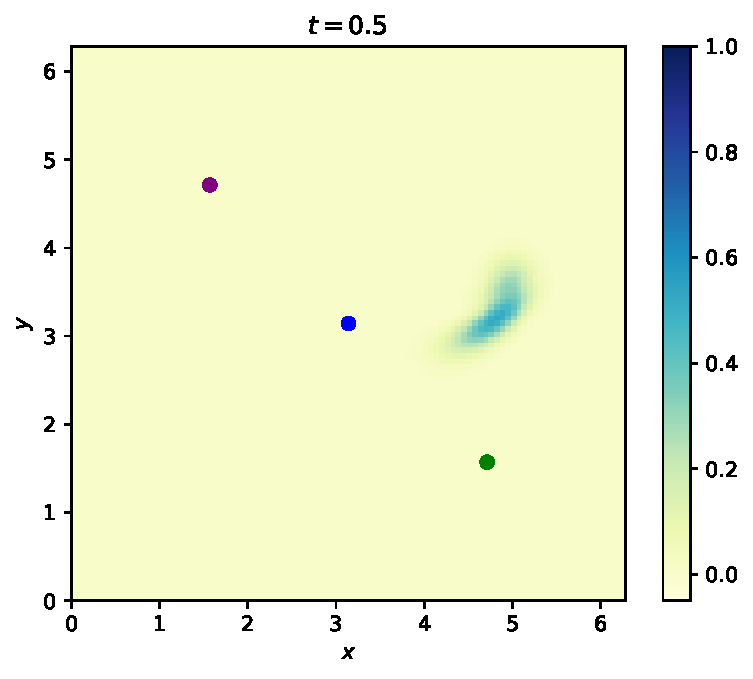
\includegraphics[width=6cm, height=6cm]{img/LFDM0_5s.pdf}
		\centering
		\caption{}
		\label{fig:tau}
	\end{subfigure}
	~
	\begin{subfigure}{0.5\linewidth}
		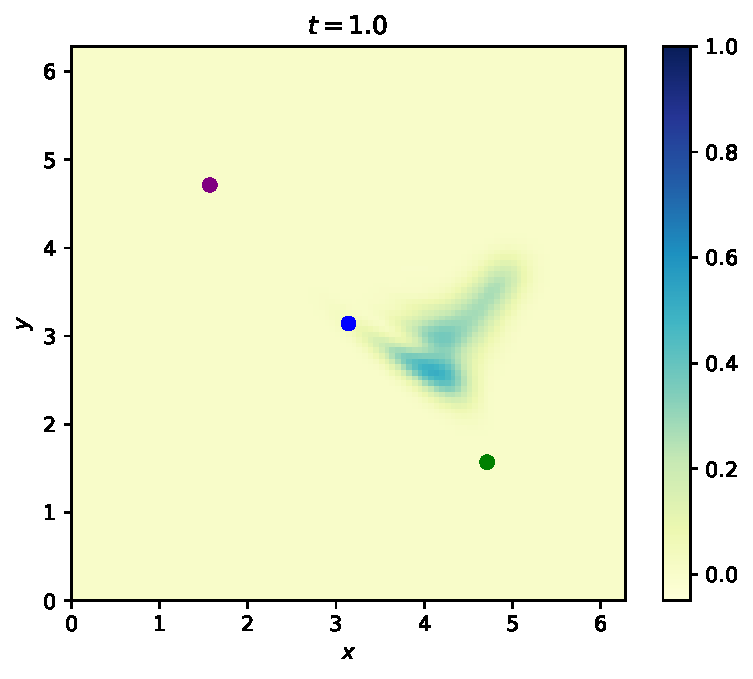
\includegraphics[width=6cm, height=6cm]{img/LFDM1s.pdf}
		\centering
		\caption{}
		\label{fig:tau}
	\end{subfigure}
	~
	\begin{subfigure}{0.5\linewidth}
		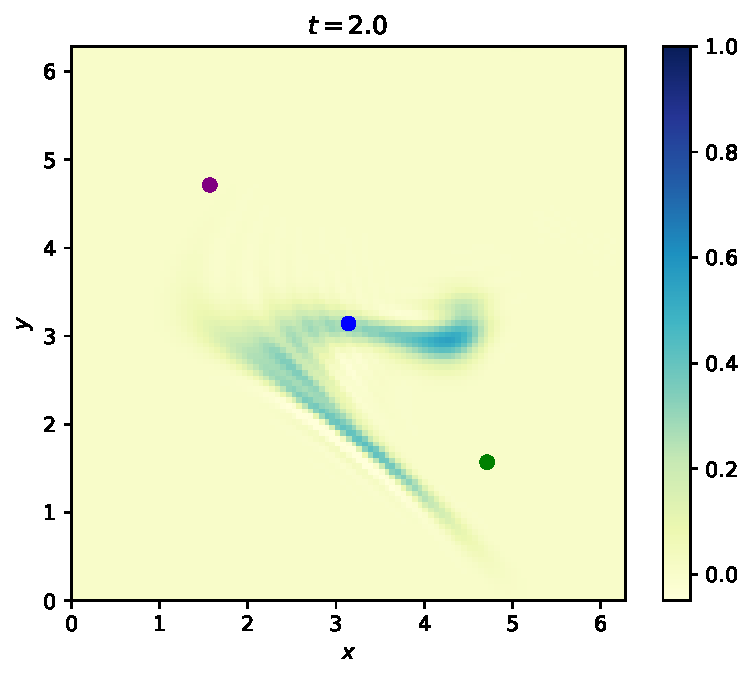
\includegraphics[width=6cm, height=6cm]{img/LFDM2s.pdf}
		\centering
		\caption{}
		\label{fig:tau}
	\end{subfigure}
	~
	\begin{subfigure}{0.5\linewidth}
		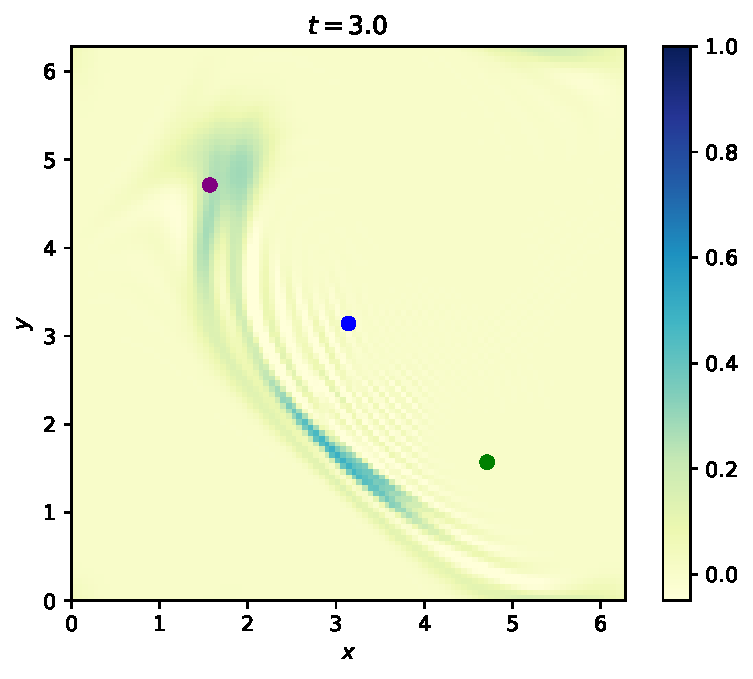
\includegraphics[width=6cm, height=6cm]{img/LFDM3s.pdf}
		\centering
		\caption{}
		\label{fig:tau}
	\end{subfigure}
	\caption{Évolution spatio-temporelle de la solution selon la méthode Leapfrog}
	\label{fig:LFDM}
\end{figure}

\begin{figure}[H]
	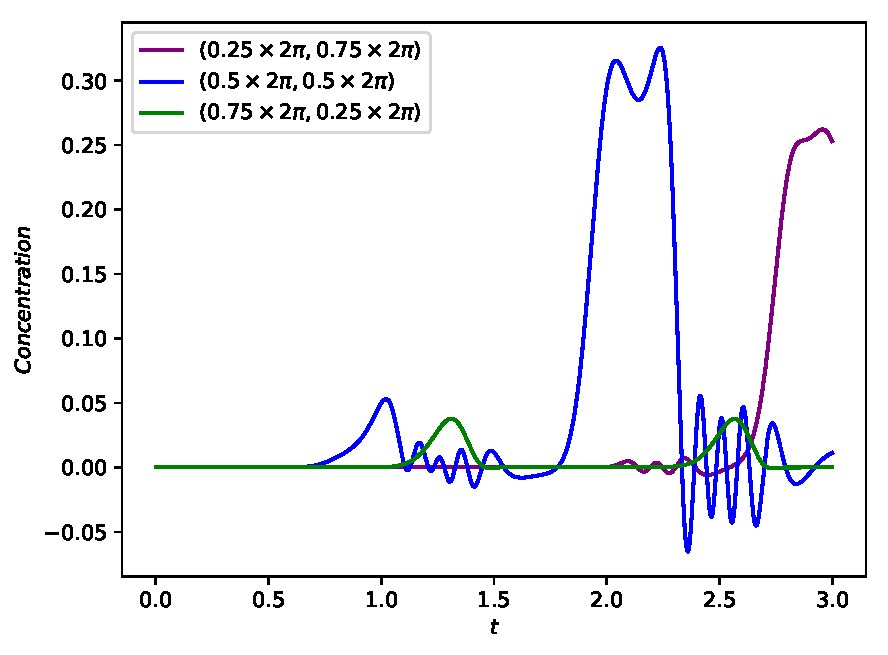
\includegraphics[width=6cm, height=6cm]{img/LFGraph.pdf}
	\centering
	\caption{Courbes de concentration en fonction du temps pour trois points de mesures selon la méthode Leapfrog}
	\label{fig:LFGraph}
\end{figure}

\subsection{Lax-Wendroff}\label{sec:LaxWendroff}

Ensuite, on confirme la calibration de l'algorithme Lax-Wendroff, encore une fois, en reproduisant les résultats affichés dans le recuil de notes de référence \cite{notes_cours}. On remarque à la figure \ref{fig:LWDM} l'affinement de la solution obtenue, entre autre dû à l'augmentation de la résolution spatiale. De plus, on remarque la diminution drastique des erreurs numériques à la figure \ref{fig:LWGraph}.

\begin{figure}[H]
	\begin{subfigure}{0.5\linewidth}
		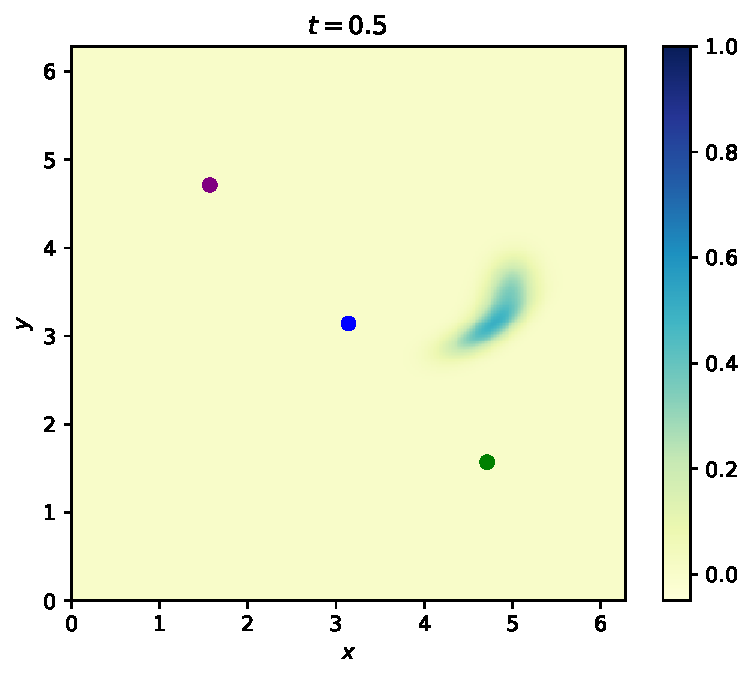
\includegraphics[width=6cm, height=6cm]{img/LWDM0_5s.pdf}
		\centering
		\caption{}
		\label{fig:tau}
	\end{subfigure}
	~
	\begin{subfigure}{0.5\linewidth}
		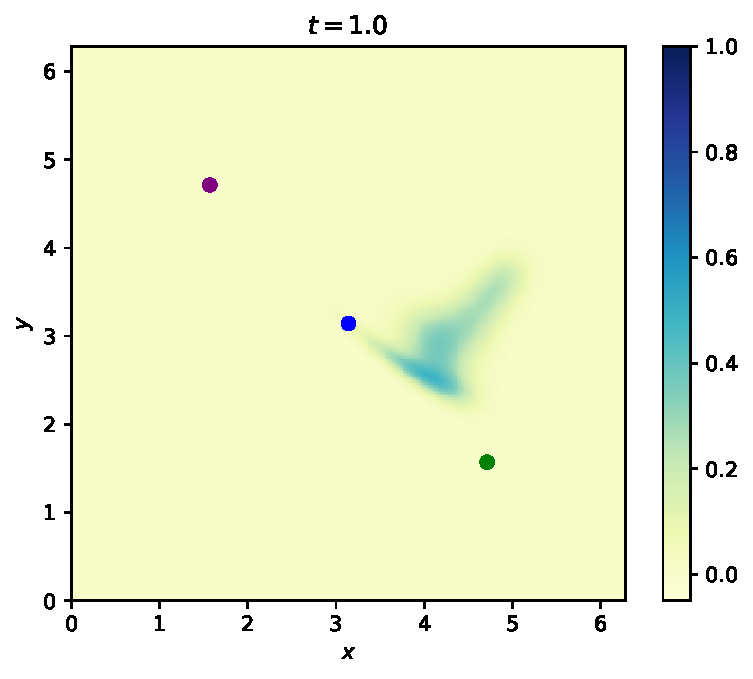
\includegraphics[width=6cm, height=6cm]{img/LWDM1s.pdf}
		\centering
		\caption{}
		\label{fig:tau}
	\end{subfigure}
	~
	\begin{subfigure}{0.5\linewidth}
		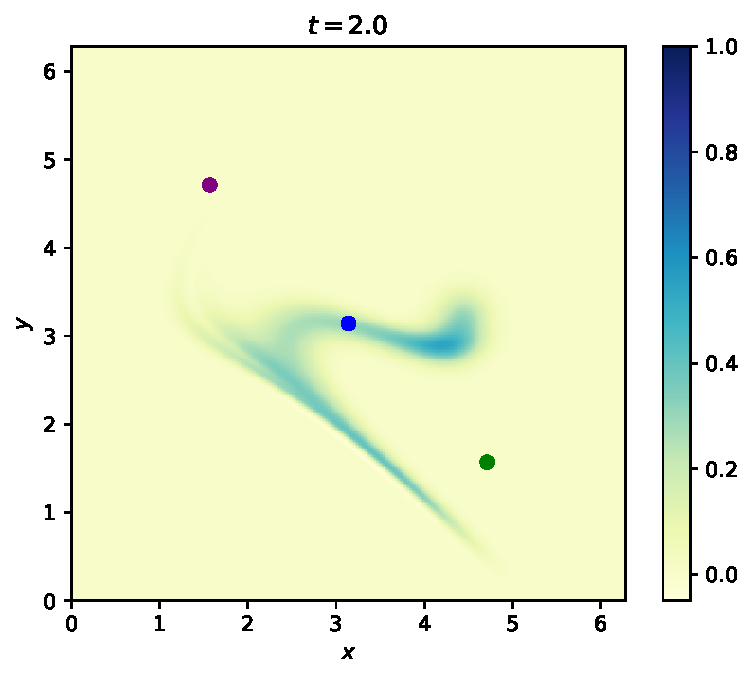
\includegraphics[width=6cm, height=6cm]{img/LWDM2s.pdf}
		\centering
		\caption{}
		\label{fig:tau}
	\end{subfigure}
	~
	\begin{subfigure}{0.5\linewidth}
		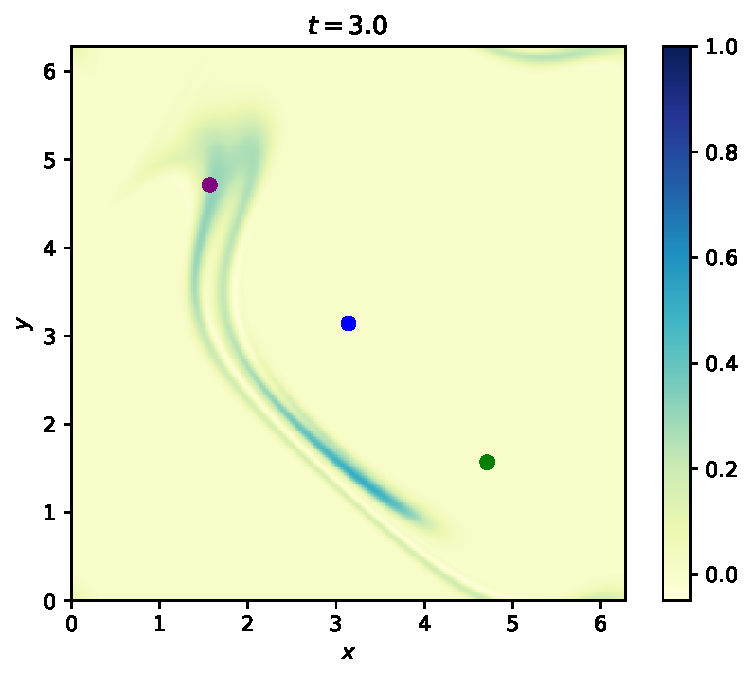
\includegraphics[width=6cm, height=6cm]{img/LWDM3s.pdf}
		\centering
		\caption{}
		\label{fig:tau}
	\end{subfigure}
	\caption{Évolution spatio-temporelle de la solution selon la méthode Lax-Wendroff}
	\label{fig:LWDM}
\end{figure}

\begin{figure}[H]
	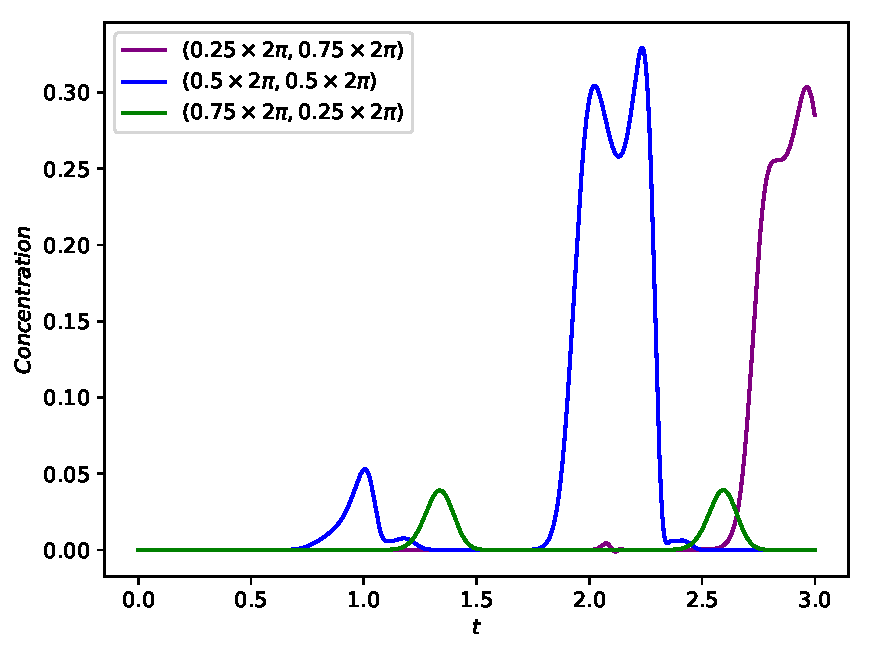
\includegraphics[width=6cm, height=6cm]{img/LWGraph.pdf}
	\centering
	\caption{Courbes de concentration en fonction du temps pour trois points de mesures selon la méthode Lax-Wendroff}
	\label{fig:LWGraph}
\end{figure}


\subsection{Détermination de la nature d'un incident}\label{sec:incident}

On est enfin prêt à déterminer la nature de la source impliquée dans l'incident fictif. La figure \ref{fig:dataGraph} affiche les données fournies, c'est-à-dire un ensemble de trois séquences temporelles de la concentration associé à trois points de mesures. Additionnellement, on nous dit que le temps d'activation de la source $t_d \in [0, 0.5]$ et que $t_f = 2.5$. 

\begin{figure}[H]
	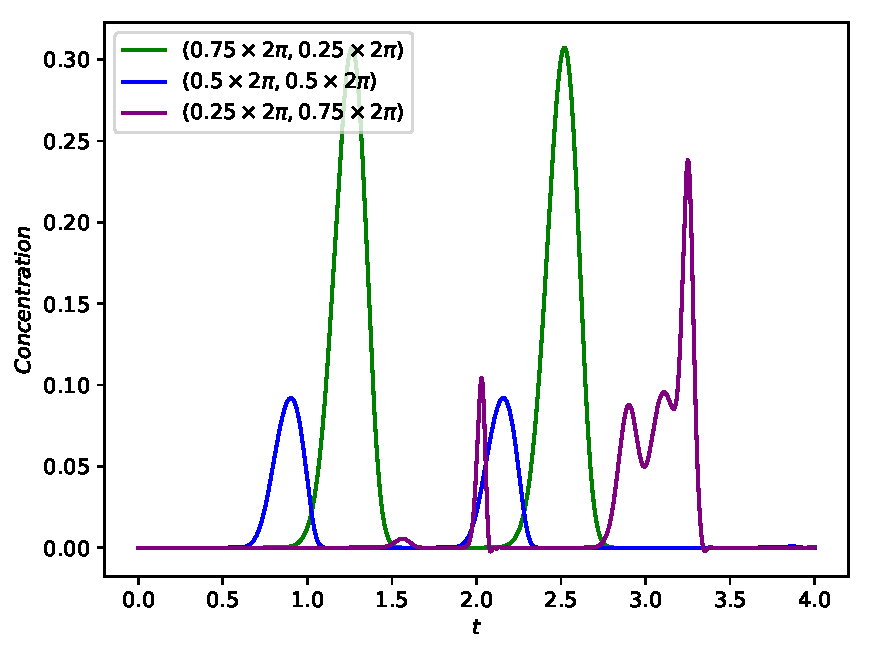
\includegraphics[width=6cm, height=6cm]{img/incidentData.pdf}
	\centering
	\caption{Données concernant l'incident}
	\label{fig:dataGraph}
\end{figure}

On commence par effectuer une étude de l'écoulement de l'air afin d'estimer grossièrement la position de la source et ainsi construire un vecteur solution initial pour la descente stochastique. En se référant à la figure \ref{fig:vents}, on remarque la présence deux zones d'écoulements périodiques. On s'attend donc à observer un taux de concentration périodique associé aux points de mesures inclus dans ces zones. En se référant à la figure \ref{fig:dataGraph} on voit que c'est le cas pour le point $(0.75\times2\pi, 0.25\times2\pi)$ et le point  $(0.5\times2\pi, 0.5\times2\pi)$. On remarque additionnellement une différence importante entre l'amplitude des courbes associées à ces deux points, ce qui suggère que la source est plus proche du point $(0.75\times2\pi, 0.25\times2\pi)$ que du point $(0.5\times2\pi, 0.5\times2\pi)$. On choisit donc la position initiale $(0.7\times2\pi, 0.4\times2\pi)$ pour la source. On construit le vecteur solution initial en choisissant une valeur intermédiaire pour $t_d$, soit de $0.25$, et une valeur de $2$ pour $S_0$.

\begin{figure}[H]
	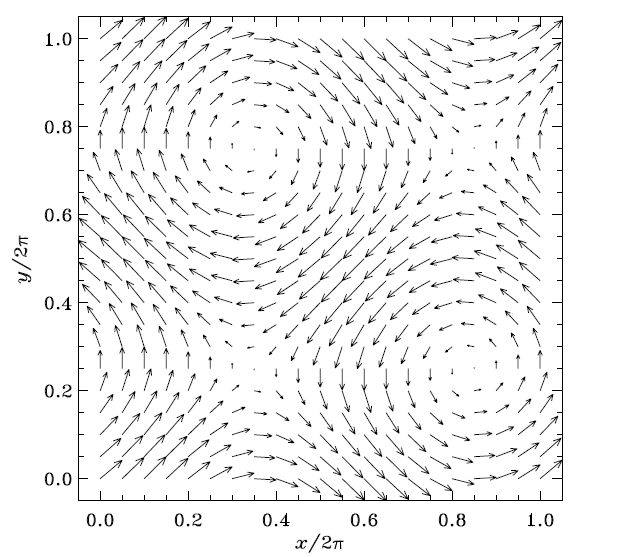
\includegraphics[width=6cm, height=6cm]{img/vents.png}
	\centering
	\caption{Écoulement de l'air \cite{notes_cours}}
	\label{fig:vents}
\end{figure}

Le vecteur solution initiale est donc $\textbf{v} = (S_0, x_0, y_0, t_d) = (2.00, 4.39, 2.51, 0.25)$. On emploie la descente stochastique Monte Carlo où la solution numérique à l'équation d'advection-diffusion est obtenue par la méthode Leapfrog. La figure \ref{fig:LFresiduals} montre la valeur de la fonction (\ref{eq:fonction_min}) après chaque itération. On observe un décroissance continuelle, ce qui démontre une convergence vers un minimum local. La descente stochastique retourne alors le nouveau vecteur solution $\textbf{v} = (1.92, 4.36, 2.63, 0.12)$. La figure \ref{fig:guessGraph} montre les résultats d'une simulation impliquant ce vecteur solution et résolu par la méthode Lax-Wendroff. Les courbes pleines représentent les données fournies tandis que les courbes pointillées représentent la solution obtenue. On observe une forte juxtaposition des courbes, ce qui suggère que la descente stochastique converge dans ce cas-ci vers un minimum global.

\begin{figure}[H]
	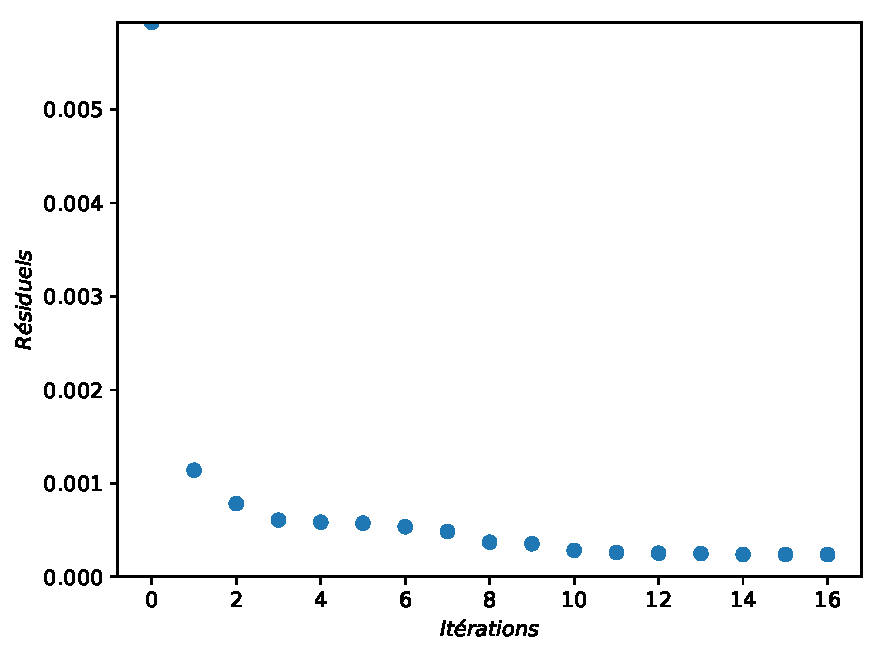
\includegraphics[width=6cm, height=6cm]{img/LFresiduels.pdf}
	\centering
	\caption{Optimisation de la fonction (\ref{eq:fonction_min}) à l'aide d'une descente stochastique Monte Carlo. La décroissance monotone représente une convergence vers un minimum local.}
	\label{fig:LFresiduals}
\end{figure}

\begin{figure}[H]
	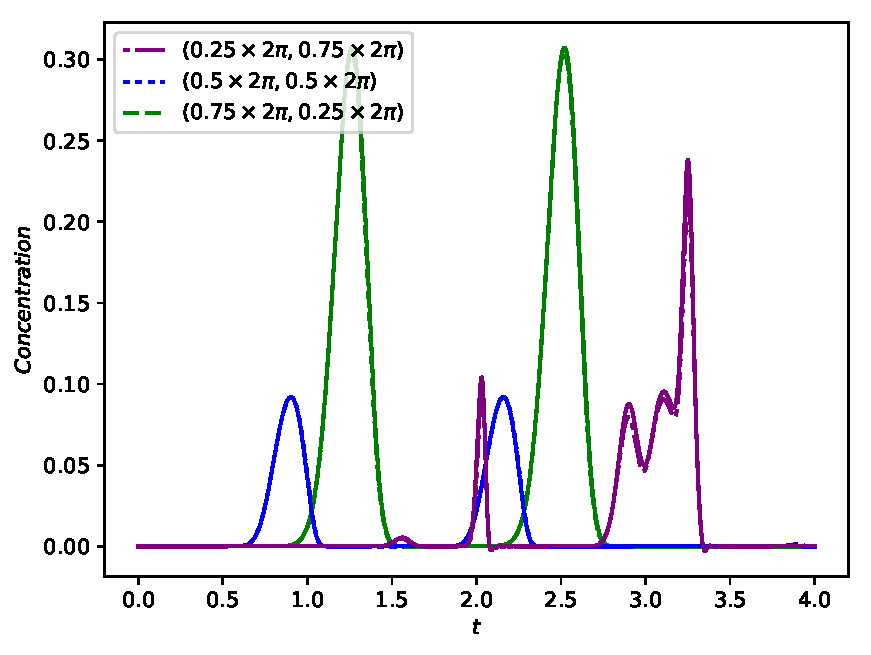
\includegraphics[width=6cm, height=6cm]{img/GuessGraph.pdf}
	\centering
	\caption{Juxtaposition des données fournies et des résultats associés au vecteur solution $\textbf{v} = (1.92, 4.36, 2.63, 0.12)$}
	\label{fig:guessGraph}
\end{figure}

Finalement, on affine les résultats en répétant la descente stochastique avec le vecteur  $\textbf{v} = (1.92, 4.36, 2.63, 0.12)$ comme point de départ mais cette fois-ci en employant la méthode Lax-Wendroff pour résoudre l'équation d'advection-diffusion. Les résultats de la descente sont affichés au tableau \ref{tab:resultats}. L'exactitude des résultats est limitée par la résolution de la maille spatiale, du pas temporel et des erreurs numériques accumulées durant le calcul de la solution. Dans le cas de Lax-Wendroff, la maille spatiale est de taille $400\times400$ et l'intervalle spatiale est de $[0, 2\pi]\times[0, 2\pi]$, ce qui se traduit en une amplitude $0.005\times\pi$ pour $\Delta x$ et $\Delta y$. Le pas temporel employé, quant à lui, est de l'ordre de $\Delta t=0.001$. Par contre, la descente stochastique s'est terminée avec un pas de grandeur de l'ordre de $h=0.00625$, ce qui engendre une borne inférieure sur l'incertitude de $t_d$. Finalement, on obtient l'incertitude sur l'amplitude de la source en prenant la déviation standard de $S_0$ au cours de la dernière descente stochastique impliquant la méthode de Lax-Wendroff.

\begin{table}[H]
	\centering
	\caption{Estimation des propriétés de la source}
	\label{tab:resultats}
	\begin{tabular}{|c|c|}
		\hline
		$S_0$ & $1.82 \pm 0.09$\\
		$x_0$ & $4.38 \pm 0.02$\\
		$y_0$ & $2.65 \pm 0.02$\\
		$t_d$ & $0.090 \pm 0.006$\\\hline
	\end{tabular}
\end{table}

\section*{Conclusion}

En utilisant deux méthodes d'analyse numérique, soient Leapfrog et Lax-Wendroff, il a été possible de solutionner le modèle d'advection-diffusion représentant la dispersion d'un polluant. En reproduisant des résultats connus, on a démontré que les méthodes employées étaient correctement calibrées et produisaient les résultats prédits par la théorie. Ensuite, on a cherché à solutionner le problème de la dispersion d'un polluant causé par un incident fictif en caractérisant la nature de la source polluante responsable . Plus précisément, on a cherché à déterminer l'amplitude $S_0$, les positions $x_0$ et $y_0$, et le temps d'activation $t_d$ de la source. En analysant initialement l'écoulement de l'air dans la région étudiée, on a grossièrement évaluer la position de la source et ainsi construit un vecteur solution initial. En employant une descente stochastique Monte Carlo et la méthode Leapfrog, on a démontré la convergence vers une solution optimale. Finalement, on a affiné notre solution en réitérant la descente stochastique Monte Carlo mais en utilisant la méthode Lax-Wendroff. On trouve un vecteur solution $(S_0, x_0, y_0, t_d) = (1.82 \pm 0.09,\ 4.38 \pm 0.02,\ 2.65 \pm 0.02,\ 0.090 \pm 0.006)$. 

\section{Bibliographie}\label{sec:bibliographie}
\begin{thebibliography}{l}
	\bibitem{notes_cours} 
	\textsc{Charbonneau}, P., Recueil de notes, Modélisation numérique en physique, Département de Physique, Université de Montréal, Janvier 2019
	
	\bibitem{notes_cours_phy1234} 
	\textsc{Charbonneau}, P., \textsc{Lafrenière}, D., Recueil de notes, Introduction à la physique numérique, Département de Physique, Université de Montréal, Automne 2016
	
	\bibitem{thermodynamics}
	\textsc{Schroeder}, D.,  An Introduction to Thermal Physics, Addison Wesley Longman, Weber State University, 2000
	
	\bibitem{github}
	\textsc{Pfleiderer}, E., Dépôt GitHub, https://github.com/EricPfleiderer/Portfolio/tree/master/PHY3075/PROJET2
\end{thebibliography}

\end{document}
